%
% Frontmatter - Introducci�n. Los miembros del tribunal que juzgan los PFC's tienen muchas m�s memorias que leer, por lo que
%	agradecer�n cualquier detalle que permita facilitarles la vida. En este sentido, realizar una peque�a introducci�n,
%	comentar la organizaci�n y estructura de la memoria y resumir brevemente cada cap�tulo puede ser una buena pr�ctica
%	que permita al lector centrarse f�cilmente en la parte que m�s le interesa.
%

\chapter[Introduction]{
	Introduction
}






Computer Graphics is the discipline that deals with creating, managing, analyzing and visualizing graphics using a computer, and it is closely linked to other disciplines such as Image Processing, Computer Vision or Machine Learning, among others. Advances in computer graphics have had an impact on several media types such as, for example, the movies and video games industry, civil engineering, medicine, etc.

In computer graphics, \emph{rendering} is the process of generating a 2D image to be shown in a display. This process takes usually a virtual scene of 3D objects as input, containing data like geometry, lighting, cameras, etc.
Typically, polygonal modeling has been the approach followed for modeling objects in the scene, approximating their surfaces using polygons. Point-based graphics focuses on points as the fundamental representation of the surfaces instead of polygons (see \figurename~\ref{poly_comp}).

\begin{figure}
	\centering
	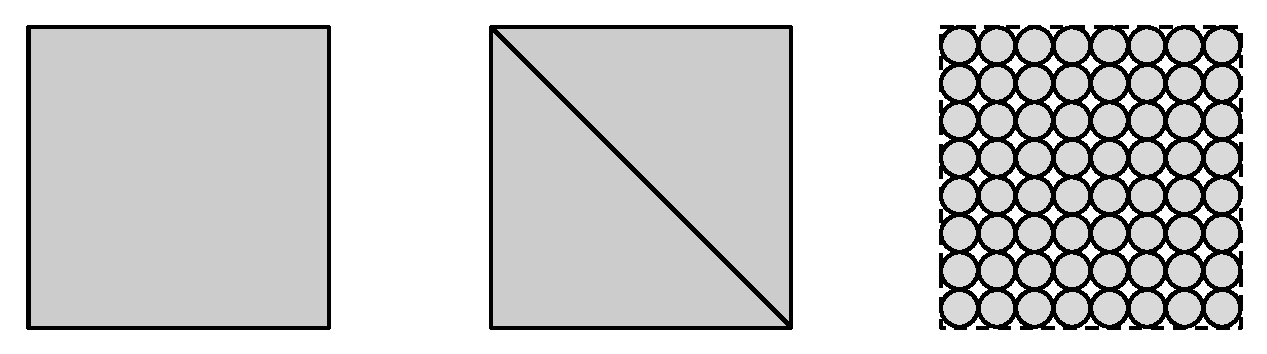
\includegraphics[scale=0.6]{figures/pol_comp.pdf}
	\caption[Modeling types comparison]{
		From left to right; mathematical representation of a plane, representation using two polygons (triangles) and a point-based representation.
	}
	\label{poly_comp}
\end{figure}

Nowadays, acquisition technologies such as LIDAR (Laser Imaging
Detection and Ranging) allow us to obtain high-precision
georeferenced 3D scans of the real world in an easy and fast way.
These systems use ultraviolet, visible or near infrared light to image objects. It can target a wide range of materials and even single molecules. A narrow laser beam can map features with very high precision.
The evolution of this kind of technologies is having a tremendous
impact in multiple fields in the engineering, and bringing back the
campwork to the office has become a standard practice.
This presents clear advantages compared to the classical work-flow in
disciplines like topography, that usually need to come back on the
ground each time a new measurement is required.

These scanning devices generate data-sets with an enormous number of
samples, with 3D coordinates and additional data such as color,
reflectivity and so on. These point clouds, as they are usually
named, are formed by hundreds or thousands of points, resulting in
Giga or even tera-bytes of information.
Using point based representations, the polygonal approximation step
can be skipped and the massive amount of captured data is directly
used. However, managing these huge data-sets, either for applying some kind of data
analysis or for visualization, is a computational challenge and an
open and state-of-the-art problem. This project deals with this question.

This chapter introduces the motivation behind the project and the
objectives we try to achieve. It shows the structure of this document
as well.

\section[Motivation and context]{
	Project motivation and context
}

PCM is a software library developed in the University of A Coru�a for the management of huge point datasets obtained by LIDAR in commodity hardware systems. It was started as a MSc Final Project~\cite{Jaspe12} (system structure and basic capabilities) in the Faculty of Computer Science and then continued in a BSc Final Project~\cite{Jaspe13} (improved render and other minor additions).

PCM is based on a multi-resolution structure and includes basic memory hierarchy management, making it possible to transfer the point cloud data between secondary memory (HDD) and video memory in the graphics card. Originally, PCM includes a very basic visualizer, quite simple and limited but that has the potential to become the seed for a more advanced point cloud software tool that will allow the user to access all of these features in real-time.

Because of the massive nature of these datasets (some of them possess more than a billion points) achieving real-time manipulation of them is a complex task. It will require the improvement of PCM and a careful performance analysis. Having a system that is able to deal with these amounts of data, will let the user take advantage of the full precision of the capture devices if needed. 

Also because of the huge amounts of data, the possibility of using the massive parallel computing power of graphics cards will be explored. The large number of parallel processors can be used to reduce the computation times as much as possible. 

In this project, a complete software tool for visualization, management and manipulation of massive 3D point clouds will be developed. The tool will be multiplatform (GNU/Linux, Windows and MacOS) and will make use of open source software. That is why for the user interface it will take advantage of QT, that has native tools for all the aforementioned platforms. The resulting QT application will let the user access all of the functionality including an advanced and complete 3D visualizer.
   

\section[Objetives]{
	Project objetives
}

The aim of this project is the design and implementation of a point-based multiplatform software tool for interactive visualization, management and manipulation of massive 3D point clouds. 

The application will offer the user the necessary tools to work effectively with this type of datasets, including a 3D visualizer with advanced point-rendering techniques using OpenGL, that will allow real time interaction with one or multiple point clouds. 

From the interface, the user will be able to:     

\begin{itemize}
\item Select different visualization modes for point-based models: multiple cameras, simple and advanced visualization, multi-resolution, etc.
\item Combine different point clouds with tools that enable rotation, translation and scaling of the clouds.
\item Select points in the clouds for working with them.
\item Apply operations to a part of the cloud or the complete dataset. From simple operations like distance measurements to plane or other geometric primitives detection.
\item Export the work done to a standard CAD format, so the tool can be integrated in other workflows. 
\end{itemize}

The developed tool will take advantage of the parallel computing possibilities of the platforms. Either using the GPGPU capabilities of the graphics card with OpenCL or the multiple cores of the CPU. 

PCM will be used as the foundation for this work. PCM is a project in development that offers several low level tools for working with point clouds of arbitrary size in commodity hardware, from which a multi-resolution structure with different levels of cache is highlighted. This final year project will not only extend PCM with the mentioned features, offering a high level tool for the final user, but will also improve the existing source code; paying special attention to performance aspects.

A series of benchmarks will also be implemented that will allow to obtain automatically and autonomously performance information about PCM and the visualization tool, with graphs and reports. This tool will make finding bottlenecks and performance issues easier.

\section[Structure]{
Document structure
}

The document is organized in the following structure.

\paragraph*{Chapter 1.}
Introduction

A brief summary of the work is presented, covering motivation, context and objetives.

\paragraph*{Chapter 2.}
Planification and methodology

We start by describing the planification and methodology used in the project.
 
\paragraph*{Chapter 3.}
Computer Graphics basics

This chapter briefs the basic concepts about computer graphics. How does the camera work and camera types, what are 3D transformations and how a point is represented in 3D.
 
\paragraph*{Chapter 4.}
Structure of a real-time visualizer for point-based datasets

This chapter describes the structure of the visualizer and presents the class diagram of the software.

\paragraph*{Chapter 5.}
PCM

The chapter explains what is PCM and what improvements were made to the library.

\paragraph*{Chapter 6.}
ToView

In this chapter we detail everything related to ToView, the software package developed from scratch in this project.

\paragraph*{Chapter 7.}
Advanced GPU point rendering

An in depth analysis of the most advanced point rendering techniques nowadays.

\paragraph*{Chapter 8.}
Object detection: RANSAC

In this chapter, an extensive explanation of the RANSAC algorithms used in this project is given.

\paragraph*{Chapter 9.}
Preprocessing and filtering

A chapter that explores the preprocessing and filtering techniques implemented in the project.

\paragraph*{Chapter 10.}
Conclusions and future lines of work

Finally, future possibilities for the project and conclusions reached during its development are exposed.
 
 




